% Diagrammes supplémentaires pour la section IA et Industrie 4.0

% Diagramme : Évolution de l'IA dans le temps
\begin{figure}[H]
\centering
\begin{tikzpicture}[
    node distance=0.8cm,
    timeline/.style={->, >=stealth, very thick, blue!70},
    event/.style={circle, draw, thick, fill=orange!30, minimum size=0.8cm, font=\tiny},
    label/.style={font=\scriptsize, text width=2.5cm, align=center}
]

% Ligne de temps
\draw[timeline] (0,0) -- (14,0);

% Événements
\node[event] (turing) at (1,0) {};
\node[label, above=0.3cm of turing] {1950\\Test de Turing};

\node[event] (dartmouth) at (3,0) {};
\node[label, above=0.3cm of dartmouth] {1956\\Dartmouth\\Naissance IA};

\node[event] (expert) at (5,0) {};
\node[label, above=0.3cm of expert] {1980\\Systèmes\\Experts};

\node[event] (backprop) at (7,0) {};
\node[label, above=0.3cm of backprop] {1986\\Back-\\propagation};

\node[event] (svm) at (9,0) {};
\node[label, above=0.3cm of svm] {1995\\SVM\\ML moderne};

\node[event] (deepblue) at (11,0) {};
\node[label, above=0.3cm of deepblue] {1997\\Deep Blue\\bat Kasparov};

\node[event] (alexnet) at (13,0) {};
\node[label, above=0.3cm of alexnet] {2012\\AlexNet\\Deep Learning};

% Périodes (en dessous)
\draw[thick, red!60] (1,-0.5) -- (3,-0.5);
\node[label, below=0.5cm] at (2,-0.5) {\textcolor{red}{Hiver 1}};

\draw[thick, red!60] (5.5,-0.5) -- (7.5,-0.5);
\node[label, below=0.5cm] at (6.5,-0.5) {\textcolor{red}{Hiver 2}};

\draw[thick, green!60] (11,-0.5) -- (14,-0.5);
\node[label, below=0.5cm] at (12.5,-0.5) {\textcolor{green!60!black}{Ère Deep\\Learning}};

\end{tikzpicture}
\caption{Chronologie des événements majeurs de l'Intelligence Artificielle}
\label{fig:ai_timeline}
\end{figure}

% Diagramme : Comparaison IA Faible vs IA Forte
\begin{figure}[H]
\centering
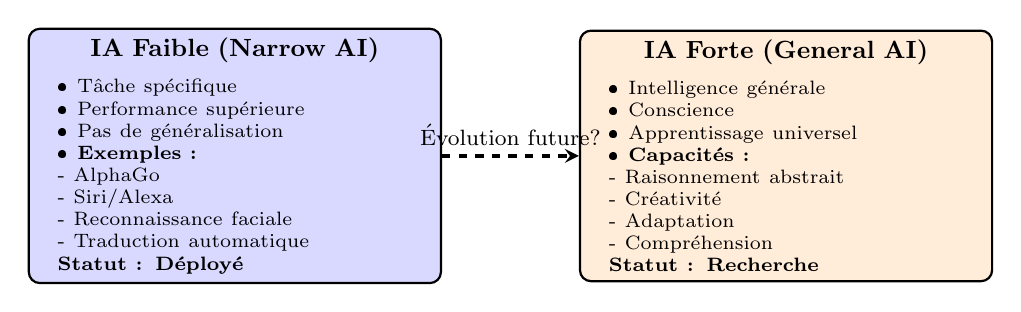
\begin{tikzpicture}[
    node distance=2cm,
    box/.style={rectangle, draw, thick, text width=5cm, text centered, rounded corners, minimum height=3cm, font=\small}
]

\node[box, fill=blue!15] (weak) at (0,0) {
    \textbf{IA Faible (Narrow AI)}\\[5pt]
    \begin{minipage}{4.5cm}
    \scriptsize
    • Tâche spécifique\\
    • Performance supérieure\\
    • Pas de généralisation\\
    • \textbf{Exemples :}\\
    - AlphaGo\\
    - Siri/Alexa\\
    - Reconnaissance faciale\\
    - Traduction automatique\\
    \textbf{Statut : Déployé}
    \end{minipage}
};

\node[box, fill=orange!15] (strong) at (7,0) {
    \textbf{IA Forte (General AI)}\\[5pt]
    \begin{minipage}{4.5cm}
    \scriptsize
    • Intelligence générale\\
    • Conscience\\
    • Apprentissage universel\\
    • \textbf{Capacités :}\\
    - Raisonnement abstrait\\
    - Créativité\\
    - Adaptation\\
    - Compréhension\\
    \textbf{Statut : Recherche}
    \end{minipage}
};

\draw[->, >=stealth, very thick, dashed] (weak) -- node[above, font=\footnotesize] {Évolution future?} (strong);

\end{tikzpicture}
\caption{Comparaison entre IA Faible et IA Forte}
\label{fig:weak_vs_strong_ai}
\end{figure}

% Diagramme : Cycle de vie d'un projet ML dans l'Industrie 4.0
\begin{figure}[H]
\centering
\begin{tikzpicture}[
    node distance=1.5cm,
    step/.style={rectangle, draw, thick, fill=blue!15, text width=2.5cm, text centered, rounded corners, minimum height=1cm, font=\footnotesize},
    arrow/.style={->, >=stealth, thick},
    feedback/.style={->, >=stealth, thick, dashed, red!60}
]

% Étapes du cycle
\node[step, fill=green!20] (collect) at (0,0) {Collecte\\Données IoT};
\node[step] (prepare) at (3,0) {Préparation\\Nettoyage};
\node[step] (train) at (6,0) {Entraînement\\Modèle ML};
\node[step] (deploy) at (9,0) {Déploiement\\Production};
\node[step] (monitor) at (6,-2.5) {Monitoring\\Performance};
\node[step] (retrain) at (3,-2.5) {Réentraînement\\Adaptation};

% Flèches principales
\draw[arrow] (collect) -- (prepare);
\draw[arrow] (prepare) -- (train);
\draw[arrow] (train) -- (deploy);
\draw[arrow] (deploy) -- (monitor);
\draw[arrow] (monitor) -- (retrain);
\draw[arrow] (retrain) -- (prepare);

% Boucle de feedback
\draw[feedback, bend right=30] (monitor) to node[right, font=\scriptsize] {Drift détecté} (train);

\end{tikzpicture}
\caption{Cycle de vie d'un système ML en production industrielle}
\label{fig:ml_lifecycle_industry}
\end{figure}

% Diagramme : Matrice de maturité Industrie 4.0
\begin{figure}[H]
\centering
\begin{tikzpicture}[
    node distance=0cm,
    level/.style={rectangle, draw, thick, text width=2.5cm, text centered, minimum height=1.5cm, font=\scriptsize}
]

% Niveaux de maturité
\node[level, fill=red!20] (level1) at (0,0) {\textbf{Niveau 1}\\Traditionnel\\Manuel};
\node[level, fill=orange!20] (level2) at (3,0) {\textbf{Niveau 2}\\Automatisé\\ERP/MES};
\node[level, fill=yellow!30] (level3) at (6,0) {\textbf{Niveau 3}\\Connecté\\IoT/Cloud};
\node[level, fill=green!30] (level4) at (9,0) {\textbf{Niveau 4}\\Intelligent\\IA/ML};
\node[level, fill=blue!30] (level5) at (12,0) {\textbf{Niveau 5}\\Autonome\\Smart Factory};

% Flèches de progression
\draw[->, >=stealth, very thick] (level1) -- (level2);
\draw[->, >=stealth, very thick] (level2) -- (level3);
\draw[->, >=stealth, very thick] (level3) -- (level4);
\draw[->, >=stealth, very thick] (level4) -- (level5);

% Indicateur position BACOVET
\node[below=1cm of level3, font=\footnotesize, text=red] (bacovet_before) {BACOVET\\Avant projet};
\draw[->, >=stealth, thick, red] (bacovet_before) -- (level3);

\node[below=1cm of level4, font=\footnotesize, text=green!60!black] (bacovet_after) {BACOVET\\Après projet};
\draw[->, >=stealth, thick, green!60!black] (bacovet_after) -- (level4);

\end{tikzpicture}
\caption{Matrice de maturité Industrie 4.0 et positionnement de BACOVET}
\label{fig:maturity_matrix}
\end{figure}

% Diagramme : Écosystème technologique du projet
\begin{figure}[H]
\centering
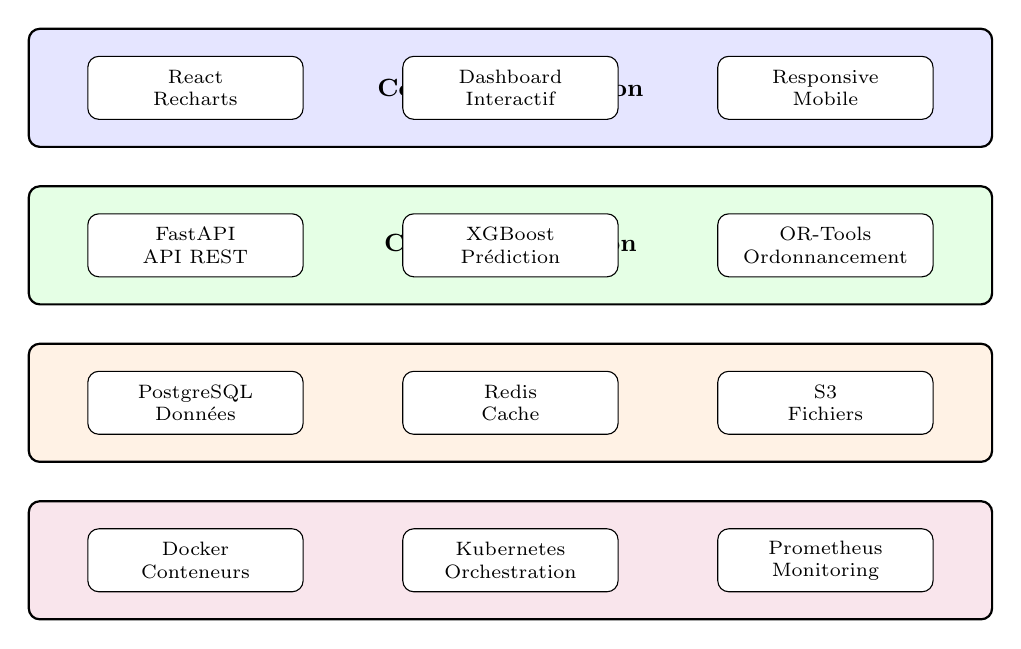
\begin{tikzpicture}[
    node distance=1.2cm,
    layer/.style={rectangle, draw, thick, text width=12cm, text centered, rounded corners, minimum height=1.5cm, font=\small},
    component/.style={rectangle, draw, fill=white, text width=2.5cm, text centered, rounded corners, minimum height=0.8cm, font=\scriptsize}
]

% Couches de l'architecture
\node[layer, fill=blue!10] (presentation) at (0,0) {\textbf{Couche Présentation}};
\node[layer, fill=green!10] (application) at (0,-2) {\textbf{Couche Application}};
\node[layer, fill=orange!10] (data) at (0,-4) {\textbf{Couche Données}};
\node[layer, fill=purple!10] (infrastructure) at (0,-6) {\textbf{Infrastructure}};

% Composants de chaque couche
\node[component] (react) at (-4,0) {React\\Recharts};
\node[component] (dashboard) at (0,0) {Dashboard\\Interactif};
\node[component] (mobile) at (4,0) {Responsive\\Mobile};

\node[component] (fastapi) at (-4,-2) {FastAPI\\API REST};
\node[component] (ml) at (0,-2) {XGBoost\\Prédiction};
\node[component] (optim) at (4,-2) {OR-Tools\\Ordonnancement};

\node[component] (postgres) at (-4,-4) {PostgreSQL\\Données};
\node[component] (cache) at (0,-4) {Redis\\Cache};
\node[component] (files) at (4,-4) {S3\\Fichiers};

\node[component] (docker) at (-4,-6) {Docker\\Conteneurs};
\node[component] (k8s) at (0,-6) {Kubernetes\\Orchestration};
\node[component] (monitoring) at (4,-6) {Prometheus\\Monitoring};

\end{tikzpicture}
\caption{Architecture technologique en couches du système}
\label{fig:tech_architecture_layers}
\end{figure}
